%-----------------------------------------------------------------------
%     Beginning of ofj-template.tex
%-----------------------------------------------------------------------
%
%     This is a topmatter template file for OpenFOAM Journal with LaTeX.
%
%     Templates for various common text, math and figure elements are
%     given following the \end{document} line.
%     This file is based on the template provided by AMS.
%
%     Some parts of this document are based on OFW16 Bye-Laws
%
%%%%%%%%%%%%%%%%%%%%%%%%%%%%%%%%%%%%%%%%%%%%%%%%%%%%%%%%%%%%%%%%%%%%%%%%

%-----------------------------------------------------------------------
%      Copyright notice
%-----------------------------------------------------------------------
%
%      Authors of papers published  in the OpenFOAM journal retain 
%      copyright and release their work under the 
%      Creative Commons Attribution-ShareAlike 4.0 International License.
%      https://creativecommons.org/licenses/by-sa/4.0/
%      Any code snippets included in the manuscript as well as submitted 
%      source code as supplementary material are subject to 
%      the GNU General Public Licence. 
%      http://www.gnu.org/licenses/gpl-3.0.html
%      Any usage of the name OpenFOAM as well as the logo is being done 
%      with the full involvement of OpenCFD, trademark holder of 
%      OpenFOAM.
%
%-----------------------------------------------------------------------

%-----------------------------------------------------------------------
%      Please do not modify the entries in this section
%-----------------------------------------------------------------------

%     Remove any commented or uncommented macros you do not use.

\documentclass[e-only,10pt,reqno]{ofj}

%     OpenFOAM-specific tensor and finite-volume notation packages
\usepackage{tensorNotation}
\usepackage{finiteVolumeNotation}

%    Other packages and commands
\usepackage{setspace}
\usepackage{lineno}
\usepackage{color}
\usepackage[dvipsnames,svgnames,x11names]{xcolor}
\usepackage{comment}
\newcommand{\comment}[1]{}  %comment not showed

\newcommand{\authorcontributions}[1]{%
\vspace{6pt}\noindent{\fontsize{9}{11.2}\selectfont\textbf{Author Contributions:} {#1}\par}}

%    \paragraph gives the same as the main body so we will remove its definition
%    \subsection and \subsubsection can be used if desired
\let\paragraph\undefined

%     Update the information is not the copyright
%     holder.
\copyrightinfo{2020}{OpenFOAM$^{\textregistered}$ Journal}
\numberwithin{equation}{section}
\newcommand{\OF}[0]{OpenFOAM\textsuperscript{\textregistered} }


%-----------------------------------------------------------------------
%      Please modify the entries in this section according to your neeeds
%-----------------------------------------------------------------------

%    Pick one of the following
\usepackage[markup=underlined]{changes} % Show changes - for writing manuscript and review
%\usepackage[final]{changes} % Final submitted version

%    In addition, comment the following line to hide the comment sections, if you do not need it
%    Please use this before submission and remove comments for review 
\includecomment{comment}

%    Define note (same as used in OFW bye-laws)
\newcommand{\note}[2][]{\added[#1,remark={#2}]{}}

%    Define note colour by author
%    If you would like to add notes, please add a line with your name here and a
%    unique colour
\definechangesauthor[color=NavyBlue]{HN} %Håkan Nilsson
\definechangesauthor[color=Green]{PC} %Philip Cardiff
% \definechangesauthor[color=Bittersweet]{JS} % John Smith

%    Please enter your OpenFOAM version
\OpenFOAMversions{\OF v20xx}
%    Please enter your repository - for final version 
\Repository{https://github.com/xxx}

\DOI{00.1000/xxx} %leave for submission

%    For review, use double spacing
\doublespacing

%-----------------------------------------------------------------------
%      The manuscript starts here
%-----------------------------------------------------------------------

\begin{document}

%-----------------------------------------------------------------------
%      An example for using comments to track changes
%      Please use these for manuscript preparation
%      Remove these comments for submission and final version
%-----------------------------------------------------------------------

%    These notes are taken from the OFW16 Bye-Laws
\begin{comment}

\section*{The actual document starts on next page. Some instructions:}

\section*{How to track changes}
\begin{itemize}
    \item Add your initials by \verb+\definechangesauthor+ above \verb+\begin{document}+.\\Pick your favourite color: \verb+https://en.wikibooks.org/wiki/LaTeX/Colors+
    \item This is how you \added[id=HN]{add} text:\\\verb+\added[id=HN]{add}+
    \item This is how you \added[id=HN, remark={comment}]{add (with comment)} text: \\\verb+\added[id=HN, remark={comment}]{add (with comment)}+
    \item This is how you \deleted[id=HN]{delete} text:\\\verb+\deleted[id=HN]{delete}+
    \item This is how you \deleted[id=HN, remark={comment}]{delete (with comment)} text:\\\verb+\deleted[id=HN, remark={comment}]{delete (with comment)}+
    \item This is how you make a note \note[id=HN]{A note}:\\\verb+\note[id=HN]{A note}+
    \item This is how you \replaced[id=HN]{replace}{relapce} text:\\\verb+\replaced[id=HN]{relapce}{replace}+
    \item This is how you \replaced[id=HN, remark={mis-spelled}]{replace (with comment)}{relapce (wthi coment)} text:\\\verb+\replaced[id=HN, remark={mis-spelled}]{relapse}{replace}+
    \item All markups can be removed by changing the header to \verb+\usepackage[final]{changes}+ later.
\end{itemize}

\newpage

\end{comment}

%-----------------------------------------------------------------------
%      Manuscript title and author description
%-----------------------------------------------------------------------


%    \title[short text for running head]{full title}
\title[\OF Journal publication]{\OF Journal publication}


%    Author information
%    Note: authors should not be defined for the review process as the review is double-blind
%    Author names should be given as initials for forenames followed by the surname: see the examples below

%    Only \author and \address are required; other information is
%    optional.  Remove any unused author tags.

%    \author[short version for running head]{name for top of paper}

%    Author one information
%\author{J. Smith}
%\address{Address1}
%\email{Emailaddress1}

%    Author two information
%\author{P. Murphy}
%\address{Address2}
%\email{Emailaddress2}

%    Add extra authors if required

%-----------------------------------------------------------------------
%      Manuscript abstract
%-----------------------------------------------------------------------

%    Abstract is required
\begin{abstract}
This is the place for an abstract.
\end{abstract}


\date{\today}

\dedicatory{}


\maketitle

%   Line numbering should be enable for review and disabled for final version
\linenumbers  

%-----------------------------------------------------------------------
%      Start introduction here and continue with additional sections
%-----------------------------------------------------------------------

\section{Introduction}

This is the place for introduction.

\subsection{Subsection}

Example text: 

We shall consider the specific transport property $\Q$ and note that its spatial and temporal variation is governed by a second-order partical differential equation (PDE), viz.\
\begin{align}
    \ddt{}(\rho \Q) + \div(\rho \Q \U) - \Gamma_{\Q}\laplacian\Q - S_\Q(\Q) = 0.
    \label{eq:genTransEq}
\end{align}
Herein, $\Q=\Q(\xt)$ is an arbitrary general intensive physical quantitity, e.g., a fluid property (scalar or tensor of any rank). Thus, \eqref{eq:genTransEq} is often referred to as generic transport equation.

\OF (Open Field Operation And Manipulation) is a flexible and mature C++ Class Library for Computational Continuum Mechanics (CCM) and Multiphysics. Its Object-Oriented-Programming (OOP) paradigm enables to \emph{mimic data types and basic operations} of CCM using top-level syntax as close as possible to the conventional mathematical notation \emph{for tensors and partial differential equations}:
\begin{lstlisting}[emph={ddt,div,laplacian}]
solve
(
  fvm::ddt(rho,Phi)
  + fvm::div(phi, Phi)
  - fvm::laplacian(Gamma, Phi)
 ==
  Sphi
);
\end{lstlisting}
Beside providing \OF code itself, spatial and temporal discretisation of Eq.\ \ref{eq:genTransEq} can be also described in a precise and concise manner using the finite-volume notation\, \cite{Weller1998} - see Tab.\ \ref{tab:FiniteVolumeNotation}.

\begin{table}
	\caption{Finite Volume Notation}
	\label{tab:FiniteVolumeNotation}
	\centering
		\begin{tabular}{p{0.3\textwidth}p{0.3\textwidth}}
		  \toprule
			  \multicolumn{2}{l}{implicit differential operators}\\
		  \midrule
			  rate of change     & $\fvmddt{\rho\q}$ \\%time derivative
			  convection term    & $\fvmdiv{F}{\q}{S}{\genFactor}$ \\
			  diffusion term     & $\fvmlaplacian{\Gamma}{\q}$ \\
			  linear part of source term & $\fvmSp{S_p}{\q}$ \\
			\hline
			  \multicolumn{2}{l}{explicit differential operators}\\
			\hline
			  temporal term      & $\fvcddt{\rho\q}$ \\
			  divergence term    & $\fvcdiv{\rho\U}{\q}{S}{\genFactor}$ \\
			  laplacian term     & $\fvclaplacian{\Gamma}{\q}$ \\
			  constant part of source term & $S_u$\\
		  \bottomrule
		\end{tabular}
\end{table}

\section{Theoretical backgroud}

Text in this section. Here is an examplary figure \ref{fig:example}.

%    Figure insertion; default placement is top; if the figure occupies
%    more than 75% of a page, the [p] option should be specified.
\begin{figure}
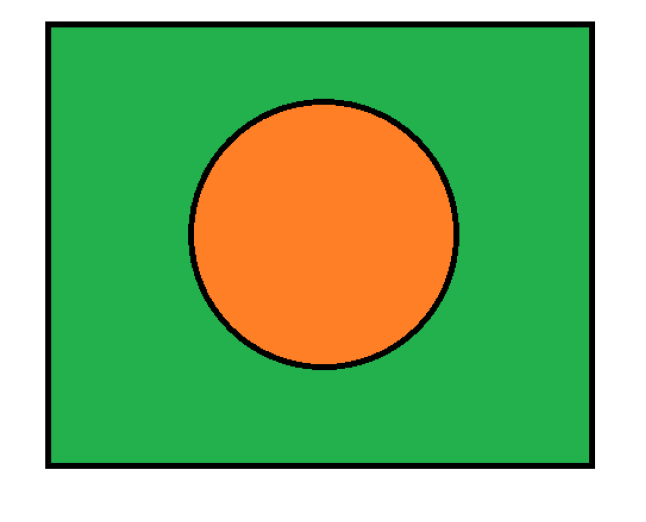
\includegraphics[width=0.5\textwidth]{example.png}
\caption{Examplary figure}
\label{fig:example}
\end{figure}


\section{Conclusion}

This is a conclusion.

%-----------------------------------------------------------------------
%      Start with acknowledgements here
%-----------------------------------------------------------------------

%\section*{Acknowledgements}
%
%This is an example acknowledgements section and should only be included !after! the review process and before publication.


% The OpenFOAM Journal requires the contributions of all authors to be explicitly stated
% As noted below, please see \href{http://img.mdpi.org/data/contributor-role-instruction.pdf}{CRediT taxonomy} for the term explanation.
% Replace the example authors initials (F.A., S.A) below as appropriate
%\authorcontributions{
%Conceptualisation, J.S.;
%methodology, J.S.;
%software, J.S;
%validation, J.S. and P.M.;
%formal analysis, J.S. and P.M.;
%investigation, J.S.;
%resources, P.M.;
%data curation, P.M.;
%writing---original draft preparation, J.S.;
%writing---review and editing, J.S. and P.M.;
%visualisation, J.S.;
%supervision, P.M.;
%project administration, P.M.;
%funding acquisition, P.M.
%All authors have read and agreed to the published version of the manuscript.
%\emph{Please turn to the  \href{http://img.mdpi.org/data/contributor-role-instruction.pdf}{CRediT taxonomy} for the term explanation.}
%}
 
%-----------------------------------------------------------------------
%      Start with appendices here
%-----------------------------------------------------------------------

% If required, include appendices here
%\appendix
%
%\section{Example appendix}
%
%This is an example appendix


%    Bibliographies can be prepared with BibTeX using IEEEtran style,
\bibliographystyle{IEEEtran}%do not change

\bibliography{Bibliography}

\end{document}

%%%%%%%%%%%%%%%%%%%%%%%%%%%%%%%%%%%%%%%%%%%%%%%%%%%%%%%%%%%%%%%%%%%%%%%%

%-----------------------------------------------------------------------
%      This is not part of the manuscript itself
%-----------------------------------------------------------------------

%    Templates for common elements of a journal article; 

%    Section headings
\section{}
\subsection{}

%    Ordinary theorem and proof
\begin{theorem}[Optional addition to theorem head]
% text of theorem
\end{theorem}

\begin{proof}[Optional replacement proof heading]
% text of proof
\end{proof}

%    Figure insertion; default placement is top; if the figure occupies
%    more than 75% of a page, the [p] option should be specified.
\begin{figure}
\includegraphics{filename}
\caption{text of caption}
\label{}
\end{figure}

% Numbered equation
\begin{equation}
\end{equation}

% Unnumbered equation
\begin{equation*}
\end{equation*}

% Aligned equations
\begin{align}
  &  \\
  &
\end{align}

%-----------------------------------------------------------------------
% End of ofj-template.tex
%-----------------------------------------------------------------------
